% article example for classicthesis.sty
\documentclass[10pt,a4paper]{article} % KOMA-Script article scrartcl
\usepackage{import}
\usepackage{xifthen}
\usepackage{pdfpages}
\usepackage{transparent}
\newcommand{\incfig}[1]{%
    \def\svgwidth{\columnwidth}
    \import{./figures/}{#1.pdf_tex}
}
\usepackage{lipsum}     %lorem ipsum text
\usepackage{titlesec}   %Section settings
\usepackage{titling}    %Title settings
\usepackage[margin=10em]{geometry}  %Adjusting margins
\usepackage{setspace}
\usepackage{listings}
\usepackage{amsmath}    %Display equations options
\usepackage{amssymb}    %More symbols
\usepackage{xcolor}     %Color settings
\usepackage{pagecolor}
\usepackage{mdframed}
\usepackage[spanish]{babel}
\usepackage[utf8]{inputenc}
\usepackage{longtable}
\usepackage{multicol}
\usepackage{graphicx}
\graphicspath{ {./Images/} }
\setlength{\columnsep}{1cm}

% ====| color de la pagina y del fondo |==== %
\pagecolor{black}
\color{white}



\begin{document}
    %========================{TITLE}====================%
    \title{\rmfamily\normalfont\spacedallcaps{Approach to binary exploitation}}
    \author{\spacedlowsmallcaps{Rodrigo Castillo}}
    \date{\today}

    \maketitle


     % ====| Loguito |==== %
    \includegraphics[width=0.1\linewidth]{negro_cara.png}
    %=======================NOTES GOES HERE===================%

    \section{Analazyng and exploiting a very very simple
    authentication program}
        for this tutorial, i made this simple script that simulates an
        authentication program:
        \begin{figure}[h!]
            \centering
            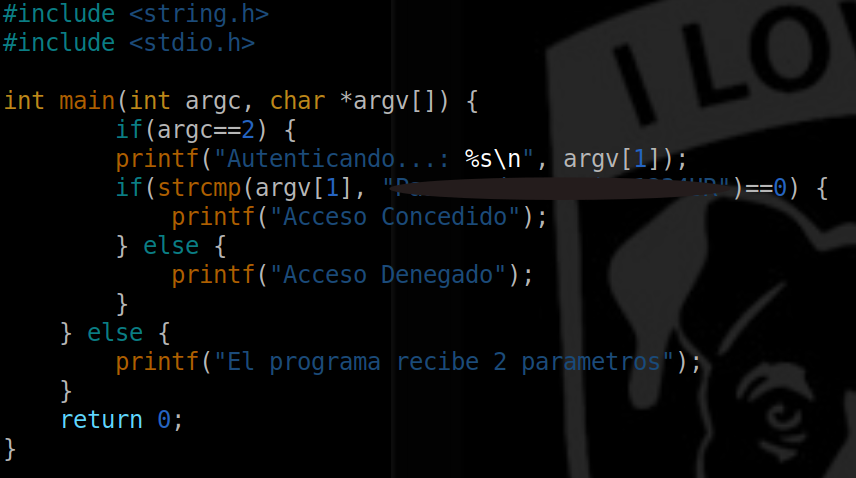
\includegraphics[width=0.8\linewidth]{very_simple_crackme.png}
            \caption{Very simple crackme}
            \label{fig:very_simple_crackme}
        \end{figure}
        \\and i compile it with $ gcc  $  compiler. the result is a binary file
        that simulates a very very simple authentication program...  as an
        atacker, i want to bypass authentication without knowing the password
        \begin{figure}[h!]
            \centering
            \includegraphics[width=0.5\linewidth]{accessdenied.png}
            \caption{Acceso Denegado}
            \label{Acceso Denegado}
        \end{figure}
        for this prupose, i previusly know many ways for bypass this security:
        \newpage
        \begin{enumerate}
            \item {Bruteforcing the password}
            \item {Debugging the binary file}
            \item {Disassembly the binary}
        \end{enumerate}

        \subsection{bruteforcing}

            Actually, we know that if the password is secure, trying to brute force
            it is going to take millions of years, so this is not an intelligent
            option, somethimes it works but just use it when is the only option
            that you have.
            \\ The second option  goes for understanding the binary file and
            modifying the flood of execution of the program, for this, we will use
            the GDB debugger, but any debugger is ok .

        \subsection{The first step is running the binary in the machine }
           \color{red}  (dont use it
            with a malware because the debugger is going to execute de binary
            file)
             \color{white}

            \begin{figure}[h!]
                \centering
                \includegraphics[width=0.8\linewidth]{disassamblyflavor.png}
                \caption{Runnig and setting GDB}
                \label{setting GDB}
            \end{figure}
            disassebly flavor intel is just because there are many assembly
            syntaxes, the most common is intel syntaxes and im used to it
            \\ first, we are going to use a disassembler for checking the functions
            that the binary file is importing
            \begin{figure}[h!]
                \centering
                \includegraphics[width=0.5\linewidth]{functions.png}
                \caption{Functions}
                \label{fig:functions}
            \end{figure}
            as we know, the "main" function is the function where the program is
            really running, the other functions like $ sym.init  $ are functions
            that the $ gcc  $ debugger is calling for compiling the $ c  $ code
            into a binary file.
            \newpage
            \\ so what we are going to do is to check the disassembly code of the $
            main  $ function.  in GDB, the command is $ disassemble  $ $ main  $ ,
            the content of this file is...
            \begin{figure}[h!]
                \centering
                \includegraphics[width=0.6\linewidth]{main.png}
                \caption{Main}
                \label{fig:main}
            \end{figure}
            understanding assembly code is, as programming, about technique and
            experience, noone reads all the disassebly code, just take a look at
            the important parts of the code... on the space $ 0x0000000000000709  $
            the program is calling the function $ printf  $ , then , there is a
            strcmp on space $ 0x0000000000000723  $ and there is a $ test  $ on the
            space $ 0x0000000000000728  $  , that means that the $ printf  $
            function is the part of the program where he is invoking the string
            "Autenticando..." and the comparisson between our input and real
            password is in the function $ strcmp@plt  $ in memory space $
            0x0000000000000723  $.
            \\
            \\ How does $ strcmp  $ works ?  its easy as assembly is working with
            processors that store numbers in hex ,  one easy way for comparing to
            strings is substracting the hex values that are stored in the
            processors ... if the result is $ 0  $ it means that the strings are
            the same, if the result is different to 0 , it means the strigns are
            different...
            \\
            \\ ones we understand previus concepts , its hacking time ...
            \\ we know that the $ strcmp  $ function is running in memory space $
            0x0000000000000723  $ and then the $ test  $ function is called, that
            means that this function is checking if the value is equal to 0 , if
            the test funcion returns false, the next instructon $ jne   $  is going
            to redirect us to $ 0x73f  $ space of memory, that means that we
            introduced a non-valid password , but if the comparisson is true, the $
            jne  $ instruction is going to let us bypass password authentication,
            for this, what we are going to do, is inserting the value $ 0  $ on the
            comparisson of the processor $ eax  $ .
            \\

            \\ first , we are going to set a breakpoint on memory space of main and run the program with the input that we want nl, in
            GDB the instruction goes with $ break$  $main  $
            \\
            \includegraphics[width=0.4\linewidth]{running.png}

            \\  with $ ni  $ we can run next intructon, so what we are going to do is walk till the
            intruction is the memory space of $ test  $ function . we can also set
            a breakpoint in the corresponding space of memory with $ break $   $
            *0x0000555555554728  $ ... running the program we can see that the way
            that we interpreted the assembly code was right ...
            \begin{figure}[h!]
                \centering
                \includegraphics[width=0.4\linewidth]{pasopaso.png}
                \caption{Pasopaso}
                \label{fig:pasopaso}
            \end{figure}
            now, we are going to keep walking till we are in the value of test function and finally...
            \\ \includegraphics[width=0.5\linewidth]{testaca.png}
            \\ We are in $ test  $ function! here, we can check the actual values
            of processors, and we can see that eax is storing the $ little $   $
            endian  $ corresponding to our input .

            \begin{figure}[h!]
                \centering
                \includegraphics[width=0.4\linewidth]{infor.png}
                \caption{info registers}
                \label{fig:infor}
            \end{figure}
            \newpage
            as we mentioned before, we need to force the $ test  $ instruction to
            return $ True  $ , so what we are going to use is set the value of $
            eax  $ to 0, in GDB the command is $ set $    $ \$eax=0  $ , then, we can
            proceed to next instructions and voila!
            \\
            \begin{figure}[h!]
                \centering
                \includegraphics[width=0.8\linewidth]{concedido.png}
                \caption{Access Granted!}
                \label{fig:concedido}
            \end{figure}
            \\
            \\
            this trick is very powerfull, because it means that we can redirect the
            flood of execution of any program and bypass its credentials!(or
            whatever we want) ,  somethimes , the process of understanding the
            way that
            programs works are a little bit more complicated but the spirit is the
            same, also, this is the most powerfull trick of this section
            because security companies encode strings and validation keys

        \newpage
        \subsection{disassemble the code}
            \newpage
            for disassemble the code, we can use any disassembler , personaly,
            i like one that is called radare2, but with in the course of
            forensics you can do it with idapro. we already know the functions
            that the program is importing, as we know, the comparisson between
            the real password and our input, is in $ main  $ function, so we
            are going to disassamble main function and check it's flood of
            execution
            \begin{figure}[h!]
                \centering
                \includegraphics[width=0.8\linewidth]{flood.png}
                \caption{Flood}
                \label{flood}
            \end{figure}
            \newpage
            here, we can see the complete flood of execution of $ main  $
            function. this is interesting, when the diagram of dlood diffuse in
            2 different diagrams, it means that there is a jump , in code, this
            can represent an $ if  $ (and sometimes a loop). the first if, is
            when the program checks if we passed 2 parameters
            \\
            \begin{figure}[h!]
                \centering
                \includegraphics[width=0.5\linewidth]{primerif.png}
                \caption{First jump}
                \label{fig:primerif}
            \end{figure}

            \\ Then, there are two options...
            \begin{figure}[h!]
                \centering
                \includegraphics[width=0.8\linewidth]{options.png}
                \caption{Options}
                \label{fig:options}
            \end{figure}
            \newpage
            if we passed correctly 2 parameters , the program send us to
            authentication, if not, print "El programa recibe 2 parámetros"
            \\ we are interested for the flood of execution of the first option...
            \begin{figure}[h!]
                \centering
                \includegraphics[width=0.7\linewidth]{floodi.png}
                \caption{Flood}
                \label{floodi}
            \end{figure}
            here, we can see that if the input is $ PasswordForensics1234UR   $ is
            going to return true and print "Acceso concedido" and if the input
            is different to $ PasswordForensics1234UR$ is going to print
            "Accesso Denegado"
            \\ that means that this is the password. this trick is powerfull
            somethimes, but normally companies compare hashes instead of plain
            text passwords, that makes the disassembling process a little bit
            more complicated, the real challenge of disassembling a binary
            comes for reversing the algorithm that makes the password return
            true .

    \section{Buffer Overflows}

    Buffer Overflow is one of the most common vulnerability in binaries out
    there, there are many types of it and it's exploitation is not intuitive at
    the beginning, but as a hacker is one of first and more important things
    that you can learn.
    \\ this is a vulnerability that was found on 80's in the golden age of
    hacking , but today there exists many problems because of this bug .
    \subsection{What is a Buffer Overflow?}
        a buffer overflow is when the program allows the user to store a custom
        variable in the stack of the memory ....
        \begin{figure}[h!]
            \centering
            \incfig{stack}
            \caption{stack}
            \label{fig:stack}
        \end{figure}
        so the problems comes when a user insert an input bigger than the
        section of memory where it is suppesed to be allowed, what really
        happens is that the input overwrite the next memory space, and this is
        very very powerfull i'll show you why in the next section ...
        \begin{figure}[h!]
            \centering
            \incfig{bof}
            \caption{bof}
            \label{fig:bof}
        \end{figure}

        \newpage
        \subsection{Exploiting a Buffer Overflow}
            for this section, i took one vulnerable machine from a guy that its
            callet $ protostar  $  , the link is here ...
            https://exploit-exercises.lains.space/download/
            \\ its a virtual machine that contains a lot of vulnerable
            exercises to practice binary exploitation
            \\ the first step is to mount the virtual machine and blah blah
            blah, we all already done that and it's the boring part of the process .
            inside the protostar's machine, in $ /opt/protostar/bin  $ there are those exercises ..
            \\
            \begin{figure}[h!]
                \centering
                \includegraphics[width=0.5\linewidth]{proto.png}
                \caption{Protostar Exercises}
                \label{fig:proto}
            \end{figure}
            in his page, we can find the source code of the exercise, an
            skilled hacker actually dont need to check the source code of the
            binary becase he can reverse it using a disassembler
            \\

            \\ we want to pwn the stack exercises , so we are going to check
            the $ stack0  $ exercise in this section just as a beginning
            example  in this section just as a beginning example.
            \\ the source code of the exercise is ...
            \begin{figure}[h!]
                \centering
                \includegraphics[width=0.5\linewidth]{source.png}
                \caption{Source Code}
                \label{fig:source}
            \end{figure}
            so the first thing we will do is to execute the binary in
            protostar's machine.
            \begin{figure}[h!]
                \centering
                \includegraphics[width=0.5\linewidth]{stack0}
                \caption{stack0}
                \label{fig:stack0}
            \end{figure}
            \newpage
            now, we are going to run the binary file with GDB debugger. as we
            can see in the source code (or in a disassembler), the program is calling for $ gets  $
            function, so we are going to check gets function .
            functions ...
            \begin{figure}[h!]
                \centering
                \includegraphics[width=0.5\linewidth]{protofun}
                \caption{functions }
                \label{fig:protofun}
            \end{figure}

            \newpage
            gets function info
            \begin{figure}[h!]
                \centering
                \includegraphics[width=0.5\linewidth]{gets.png}
                \caption{Gets}
                \label{fig:gets}
            \end{figure}

            in the description of this function we can see the string " Never
            Use this Function  " , this is because gets function is vulnerable
            to buffer overflows attacks that can let the attacker gain control
            of the machine.
            if we check the bugs section, it says
            \begin{figure}[h!]
                \centering
                \includegraphics[width=0.4\linewidth]{bug.png}
                \caption{Bug}
                \label{fig:bug}
            \end{figure}
            so we are going to exploit the buffer overflow in function $
            gets...  $ ,we are going to search the function in the disassembly
            of main function

            \begin{figure}[h!]
                \centering
                \includegraphics[width=0.4\linewidth]{protomain.png}
                \caption{Main}
                \label{fig:protomain}
            \end{figure}
            and now we know that the program is calling puts function in $
            0x804840c  $  , we want to know what is happening after this space
            of memory, so we are going to set a new breakpoint in this space of
            memory  or walk till this point with $ ni  $ command.
            \\
            \begin{figure}[h!]
                \centering
                \includegraphics[width=0.4\linewidth]{tryagain.png}
                \caption{Tryagain}
                \label{fig:tryagain}
            \end{figure}
            now, we know the point where the program is comparing the instruction.
            \\ now we execute it again but check the registers after $ 0x804840c  $
            \\
            but now, i'll put an input bigger than $ 64Bytes  $ to exploit it
            \begin{figure}[h!]
                \centering
                \includegraphics[width=0.5\linewidth]{exploited.png}
                \caption{Exploited}
                \label{fig:exploited}
            \end{figure}
            and Boom! we modified the next variable called $ modified  $ in the
            source code of the program! too powerfull!
            \\ now that we understand the concept, lets make it easy , we are
            going to make a simple python script that is going to run something
            bigger than 64 bytes and is going to pipe it into the program
            \begin{figure}[h!]
                \centering
                \includegraphics[width=0.5\linewidth]{exploitpy.png}
                \caption{Exploit}
                \label{fig:exploitpy}
            \end{figure}

            \\ and now executing the exploit ...
            \begin{figure}[h!]
                \centering
                \includegraphics[width=0.5\linewidth]{booom.png}
                \caption{Program Cracked}
                \label{fig:boom}
            \end{figure}
            actually, this is an example of the beginning of a buffer overflow,
            but this vulnerability can let an skilled hacker to gain control
            over the machine , here, in protostar page there are many examples
            of codes that can let you fall into a buffer overflow . one of the most interestings are...
            \begin{figure}[h!]
                \centering
                \includegraphics[width=0.5\linewidth]{redirectfunctions.png}
                \includegraphics[width=0.5\linewidth]{solo.png}
                \caption{Redirect functions or get full controll of the victims machine}
                \label{fig:redirectfunctions}
            \end{figure}

    \section{conclusion}
        Debuggers and Disassemblers  are tools for forensics and designed to
        understand programs, however, they have many uses and one of them is
        hacking, attackers use those tools to understand programs and exploit.
        \\ Sometimes, those attacks requiere habilities and practice , mostly
        they are made for making jokes or competitions or by bug bounters,
        but sometimes , there are people who have the same abilities and use it
        for breaking into companies , bypassing security systems and making
        in general, thats why understanding tools like mentioned before, can
        take us to perform better security systems.























    %=======================NOTES ENDS HERE===================%

    % bib stuff
    \nocite{*}
    \addtocontents{toc}{\protect\vspace{\beforebibskip}}
    \addcontentsline{toc}{section}{\refname}
    \bibliographystyle{plain}
    \bibliography{../Bibliography}
\end{document}
